\section{Gestion du projet}
    Le but de la I4-2 est de nous initier à une meilleure gestion des projets (informatiques ou non) que nous pourrions être amenés à réaliser dans le futur. En effet, un projet réussi est un projet organisé. Il convient alors de trouver un moyen de partager les codes sources et de se répartir le travail à travers tout le groupe de la manière la plus efficace. Pour tous les membres de notre groupe nous avions utilisé \verb|Google drive| lors du projet informatique du semestre 3. Nous avions alors tous eu les même problèmes pour se partager le code source et travailler en collaboration. Nous nous retrouvions chacun avec des versions différentes et du code qu'il fallait fusionner à la main ce qui faisait perdre beaucoup de temps. Nous avons donc utilisé le logiciel \verb|Git| pour ce projet qui nous a permis d'avoir un dépôt de codes sources décentralisé et de travailler efficacement.
   
    \subsection{Git et GitLab}
      
        \begin{figure}[!ht]
        
            \centering 
            
\includegraphics[width=0.2\textwidth]{images/git-logo-.jpg} 
            \caption{Logo du logiciel Git.}
            \label{logo_Git}
            
        \end{figure}
      
        \paragraph{Git}
            C'est un logiciel Open source et collaboratif de gestion de versions décentralisé. Il inclut un ensemble d'outils logiciels pour mémoriser et retrouver différentes versions d'un projet et faciliter le travail collaboratif. Nous n'utilisons pas directement \verb|Git| mais passons par un service d'hébergement Web nommé \verb|GitLab|.
      
       \begin{figure}[!ht]
        
            \centering 
            
\includegraphics[width=0.35\textwidth]{images/gitlab-logo.png} 
            \caption{Logo GitLab.}
            \label{logo_GitLab}
            
        \end{figure}
        
        \clearpage
        
        \paragraph{GitLab}
            C'est une application Web basée sur Git proposant les fonctionnalités de Git ainsi que quelques unes de ses propres fonctionnalités comme un wiki ou un système de suivi des bugs. Il permet d'avoir un dépôt virtuel, en libre accès pour chaque membre du groupe du projet. Chaque membre doit être intégré au projet pour pouvoir y participer. Le dépôt distant est cloné sur la machine réelle de l'utilisateur (commande \verb|git clone|). Par la suite, il peut modifier le dépôt, puis mettre en ligne ses modifications (commande \verb|git add|/\verb|git commit|/\verb|git push|) ou bien mettre à jour son dépôt local (commande \verb|git pull|). L'utilisation en local de \verb|GitLab| se fait par l'intermédiaire du terminal et des commandes git. Le dépôt est également accessible depuis une page Web proposant une interface graphique soignée (figure~\ref{Dépôt_GitLab}). 
        
        \vspace{1 cm}
        
        \begin{figure}[!ht]
        
            \centering 
            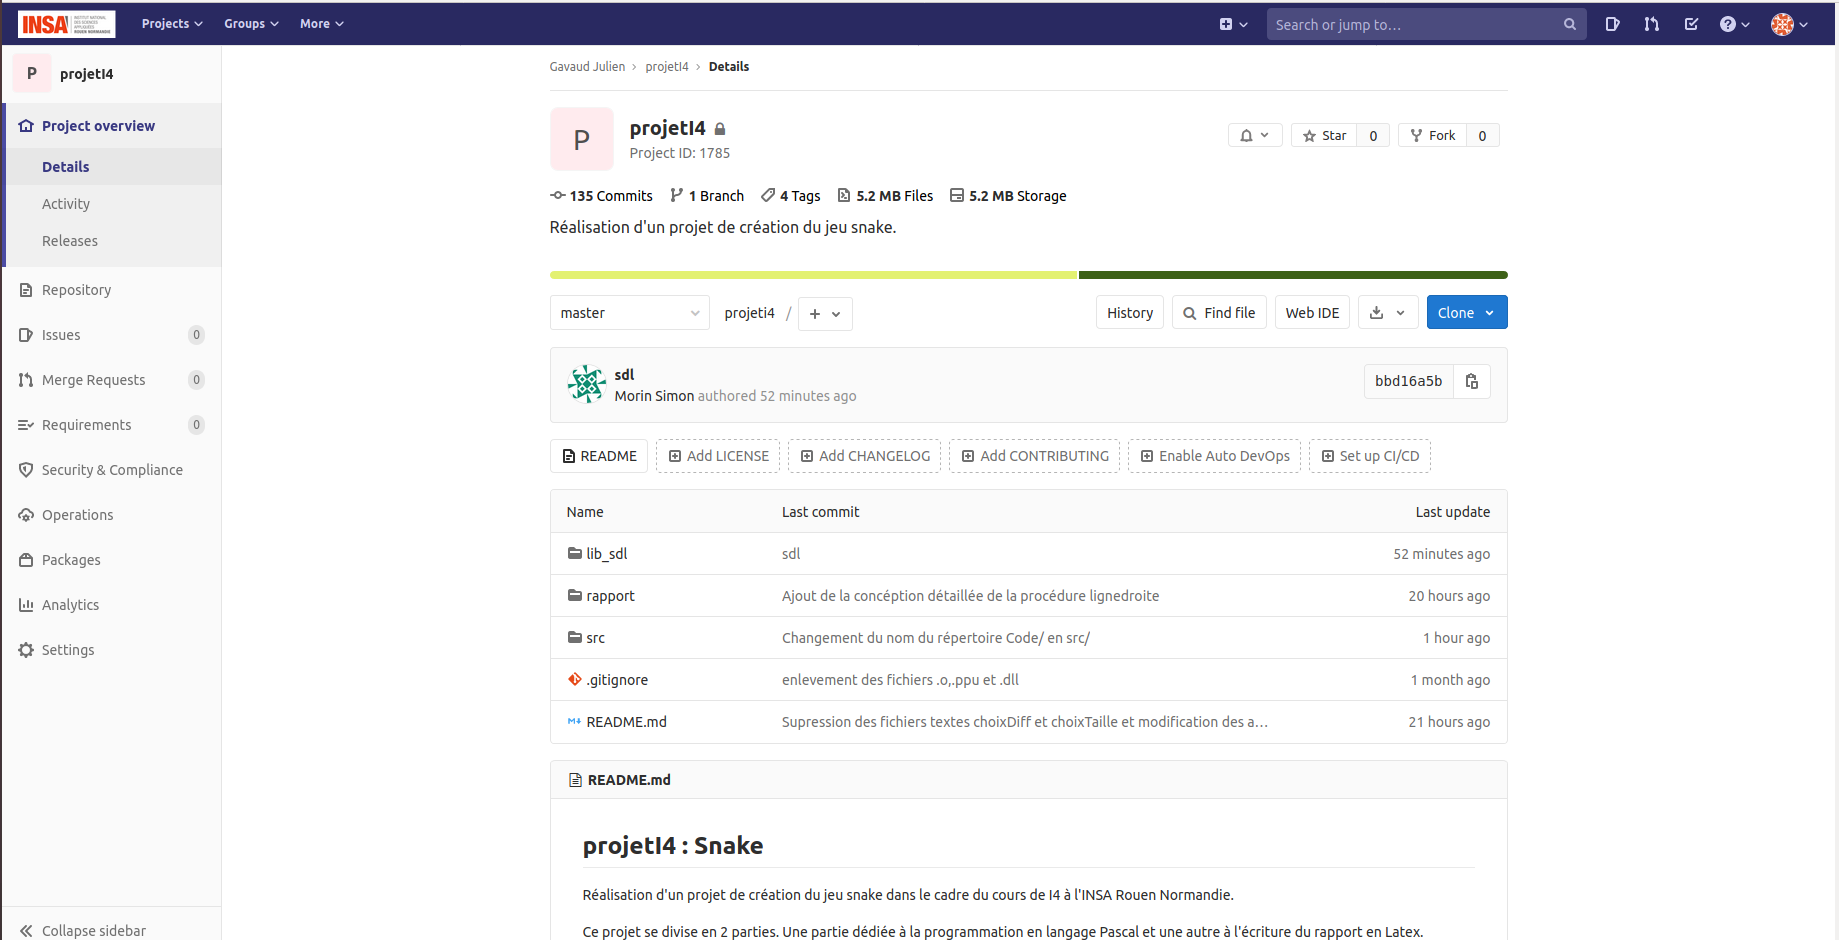
\includegraphics[width=1\textwidth]{images/depot_GitLab.png} 
            \caption{Dépôt GitLab.}
            \label{Dépôt_GitLab}
            
        \end{figure}
        
        \clearpage
        
        \subsection{Travail de groupe}
            L'intérêt de GitLab est donc de faciliter la travail de groupe. Chaque membre peut apporter sa contribution au projet, au moment où il le souhaite, et partager facilement son travail sans avoir à s'échanger des documents par mail ou autre.
        
            \subsubsection{Répartition des tâches}
                La répartition des tâches à été réalisée au bout de la troisième semaine de TD. En effet, au début, nous réfléchissions à la structure du programme tous ensemble et nous écrivions le cahier des charges du projet. Après avoir défini les grandes lignes du projet et consulté M. Baert, nous avons décidé de nous répartir les tâches pour être le plus efficace possible. La répartition s'est faite en fonction des envies et des compétences de chacun. Kevin Gatel et Simon Morin ont principalement travaillé sur le codage Pascal tandis que Julien et Théo ont codé quelques procédures Pascal mais ont plus travaillé à coder le rapport en \LaTeX. Bien évidemment, nous nous réunissions régulièrement par visio-conférence pour travailler ensemble et faire des points sur l'avancement du projet. Malgré le confinement, nous n'avons pas eu de mal à travailler ensemble grâce à Discord où nous pouvions partager nos écrans pour travailler à plusieurs. 
                
                Les deux derniers membres du groupe Hengshuo et Yizhen n'ont pas participé au projet, notament car nous n'avons eu aucun contact avec eux depuis le confinement. Nous comprenons les difficultés liées à celui-ci et à l'éloignement géographique mais nous avons été étonné de ne recevoir aucune réponse à nos nombreux messages, ne serait-ce que pour savoir s'ils pouvaient et/ou comptaient nous aider.
        
            \subsubsection{Retour d'expérience}
                Il paraît évident que nous avons rencontré plusieurs difficultés au cours de ce projet, que ce soit par rapport à l'algorithmique, au codage en \verb|Pascal|, en \verb|Latex| ou bien lors de l'utilisation de \verb|GitLab|.
            
                \paragraph{Algorithmique et Pascal} 
                    C'est la création des procédures gérant les fonctions de déplacement du serpent qui nous ont demandé le plus de réflexion. C'est le cœur du jeu et nous voulions que les déplacements soient le plus fluide possible. Au début du projet, nous travaillions avec des variables tête et queue qui étaient des coordonnées et corps qui était un tableau de type coordonnée. Comme le code était laborieux, nous avons décidé de redéfinir nos types et de créer un seul tableau comprenant toutes les coordonnées. Cela nous a fait changer beaucoup de choses dans notre projet qui était déjà bien avancé mais c'était nécessaire. 
                    Les délais d'apparition des pommes et des pommes dorées n'ont pas été faciles à programmer non plus. Nous voulions que la durée soit la même peu importe la vitesse du serpent et ça sans utiliser la fonction \verb|GetTime|. 
                    
                    Dans l'ensemble, ce projet nous a fait progresser en algorithmique. Nous nous sommes aussi rendu compte que nous avons encore de grosses marges de progressions. La prochaine étape est d'utiliser les pointeurs qui nous auraient sûrement permis d'obtenir un rendu encore meilleur. 
            
                \clearpage
                
                \paragraph{Git} 
                    Tout d'abord, lors de la première séance, nous avons modifié nos noms sur la page de garde et utilisé les mêmes lignes de texte. Ainsi, des merges apparaissaient et cela nous a permis de comprendre le fonctionnement de ce logiciel et les problèmes que nous allions pouvoir rencontrer. Celui-ci effectue une fusion des deux versions entrées en remplaçant les lignes modifiées par les utilisateurs. Seulement, si deux lignes sont toutes les deux modifiées, nous rencontrons un problème de merge. Pour résoudre ce merge nous devons modifier manuellement les lignes d'erreur. Ce problème a été assez difficile à gérer lors des premières séances. Nous ne comprenions pas comment fusionner les documents et résoudre les merges.
            
                    Néanmoins, au fur et à mesure, nous avons réussi à résoudre ces erreurs assez facilement. Nous nous organisions également pour ne pas travailler en même temps sur les mêmes choses pour éviter ces problèmes. 
            
                    Nous avons réellement essayé de nous approprier le service GitLab. Nous avons par exemple créé des clés ssh pour ne plus  avoir à nous connecter à chaque push/pull. Nous avons créé des issues sur GitLab ce qui permet de s'organiser sur les tâches restantes. GitLab possède de nombreuses fonctionnalités qu'il nous reste encore à découvrir lors de prochains projets.
            
                \paragraph{Rapport et \LaTeX}
                    Le langage d'écriture que nous avons utilisé est le \LaTeX. Cette écriture permet une présentation propre et soignée. L'avantage du \LaTeX est de permettre à l'utilisateur de se concentrer sur le contenu et non sur la forme. La mise en page est définie une fois au début du projet (ici fournie dans le document \textit{classeRapport}) et ensuite, c'est automatique. Cet aspect nous a beaucoup plu, car nous sommes tous d'accord pour dire qu'un des passages les plus pénibles lors de l'écriture d'un rapport est la mise en page. Une des grandes forces du \LaTeX est également le rendu des équations mathématiques et des algorithmes. Nous avons découvert cela pendant ce semestre et d'autant plus grâce au confinement et les cours à distance. C'est une découverte qui va nous servir pour la suite car écrire des formules sur \verb|Word| n'est pas l'idéal ... 
                    
                    Pour ce qui est des algorithmes le rendu est très satisfaisant, mais leur écriture n'est pas aisée. Nous avons eu des difficultés avec le package \verb|Algorithm2e|. Par exemple, un algorithme faisant plus d'une page "disparaît" à la fin de celle-ci sans s'écrire sur la suivante. Malgré nos recherches nous n'avons pas trouvé de moyens de résoudre ce problème. 
                    L'apprentissage est donc au début complexe, il existe une variété de commandes élévée. Nous avons souvent eu le sentiment de ne pas pouvoir profiter pleinement des possibilités qu'offre le \LaTeX. Rien que d'insérer une image sur la page de garde nous a posé problème. Les indications pour résoudre les problèmes de compilation ne sont pas toujours explicites et cela prend souvent du temps avant de trouver ce qui ne va pas. Par exemple, nous avons cherché pendant près d'une heure pourquoi le rapport ne compilait pas, pour se rendre compte que l'erreur venait d'une majuscule manquante (pour écrire le mot \LaTeX "stylisé" et pas Latex). 
            
                    Seulement, après de nombreuses heures de pratique, cela devient plutôt rapide et permet un rendu de qualité. Le \LaTeX n'est pas facile à prendre en main, mais une fois que l'on a fait cet effort on y voir réellement de nombreux avantages.

                    \clearpage
                    
                    Nous avons utilisé deux éditeurs de texte différents : 
                    
                \begin{itemize}
                    \vspace{0,2 cm}
                    
                    \item Kile pour Kevin, Simon et Julien. Kile est un éditeur minimaliste et peut se montrer assez destabilisant lors des premières utilisations.
                    \item Overleaf pour Théo. Son utilisation est simple et la page est assez design. De plus, je réutiliserai ce compilateur de \LaTeX car les erreurs de compilation empêche rarement la création du pdf. 
                    
                    \vspace{0,2 cm}
                \end{itemize}

            \par
                Néanmoins, des erreurs de compilation pouvait apparaître lors d'un passage à l'autre entre les éditeurs, ce qui était parfois ennuyeux.
                
            \subsubsection{Avis sur Git}
                \begin{itemize}
                    \item Théo : \enquote{GitLab est pour moi un excellent outil pour rassembler tout les codes sources, que ce soit du \LaTeX ou du Pascal. Les commandes utilisés à partir du Terminal permettent une utilisation fluide et rapide. On peut ainsi facilement voir les avancées qui ont été réalisées par les autres membres, via le 'poids' de chaque modification. Seulement, les problèmes de merge nuisent énormément à ce système. En effet, il faut alors soit écrasé une des deux parties, soit passer un temps fou à reprendre à la main. La gestion automatique des problèmes de fusion des fichiers ou une interaction simplifié avec l'utilisateur rendrait le logiciel bien plus utile et indispensable.}
        
                    \vspace*{0,4 cm}
        
                    \item Julien : \enquote{J'ai vraiment apprécié la découverte du logiciel Git. Une fois la prise en main effectuée j'y vois de réels avantages. Bien que je ne veuille pas aller en ASI/ITI, je pense que Git pourrai me servir dans le futur pour des rapports écrits (en \LaTeX ou autres). Le problème est que je me demande si je pourrai réutiliser le logiciel étant donné que la majorité des personnes ne connaissent pas Git. Concernant le \LaTeX, j'apprécie le rendu et les possibilités qu'offre le langage mais je ne pense pas le réutiliser sous la forme de code source dans un futur proche. En revanche, cela me donne envie d'utiliser des logiciels comme LyX.}
        
                    \vspace*{0,4 cm}
        
                    \item Kevin : \enquote{Gitlab est une plateforme en ligne permettant de synchroniser nos fichiers. Il a été d'une grande utilité notamment grâce à son utilisation assez simple et rapide, les fichiers communs sont modifiés simplement grâce à quelques lignes de commande sur le terminal. Le simple bémol serait sur les petits problèmes survenant un peu aléatoirement, nous obligeant à recloner le projet. Dans l'ensemble gitlab m'a convaincu et je l'utiliserai de nouveau pour un projet futur.}
        
                    \vspace*{0,4 cm}
        
                    \item Simon : \enquote{Je pense que GitLab est très pratique pour stocker et partager des fichiers. Il permet de synchroniser rapidement le contenu de nos dossiers, avec le dépôt en ligne, sans perdre de temps à devoir créer des archives et à se les transférer entre membres du projet. Il permet aussi de voir en ligne les modifications faîtes, de commenter des lignes de codes pour l'améliorer, et de créer des 'tâches' pour résoudre des problèmes, ce qui est plutôt cool. Le plus important est de ne pas partager un code source qui ne compile pas sinon une partie du dépôt est corrompue et c'est la croix et la bannière pour corriger les erreurs (surtout si c'est une autre personne qui a écrit le code).}
        
                \end{itemize}
                
                \clearpage

